\section{Relación}
\label{sec:relacion}

En las \texttt{Secciones \ref{sec:atributo}}, \texttt{\ref{sec:metodo}} y
\texttt{\ref{sec:clase}} se definieron los componentes clave que permiten
sistematizar la generación de código para los componentes base de los
diagramas de clase, en ésta sección, se describe un componente que permite
la asociación de diferentes clases dentro de un modelo, una \texttt{Relación}.

Estas relaciones permiten la asociación entre dos clases. Director permite
definir una sección en la cual se pueden definir un conjunto de relaciones que
luego se tendrán en cuenta a la hora de generar los componentes que se
definieron en el modelo.

La notación BNF para las relaciones es la siguiente:

\begin{lstlisting}[caption={BNF - Relationships}, basicstyle=\footnotesize\ttfamily]
  <relationships> ::= "relationships {" <lista-relaciones> "}"
\end{lstlisting}

\begin{figure}[H]
	\centering
	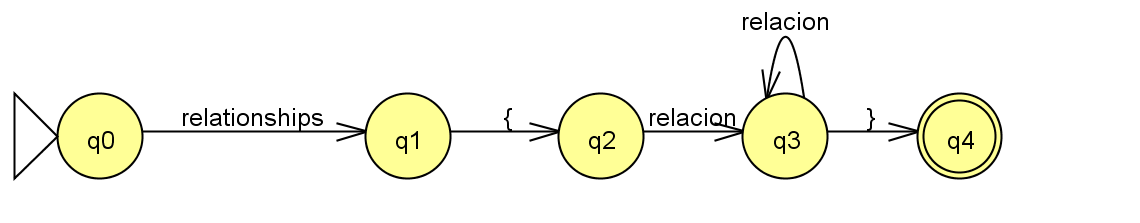
\includegraphics[width=.4\linewidth]{automatas_finitos/relationshipsDrt.png}
	\caption{Autómata finito - Relationships}
	\label{fig:relationships}
\end{figure}

en donde \texttt{lista-relaciones} se define de la siguiente manera:

\begin{lstlisting}[basicstyle=\footnotesize\ttfamily]
  <lista-relaciones> ::= <relacion> | <lista-relaciones>
\end{lstlisting}

y además se tiene que \texttt{relacion} se define de la siguiente manera:

\begin{lstlisting}[caption={BNF - Relación}, basicstyle=\footnotesize\ttfamily]
	<relacion> ::= <rol-asoc><cardinalidad>
	               <tipo-relacion>
								 <cardinalidad><rol-asoc>
\end{lstlisting}

Se debe realizar la definicion de \texttt{rol-asoc}, \texttt{cardinalidad} y
\texttt{tipo-relacion}.

\subsection*{Definición \texttt{rol-asoc}}
Se procede a definir el significado de \texttt{rol-asoc}, que lo que representa
es el rol que cumple la clase en la relacion a establecerce.

\begin{lstlisting}[caption={BNF - Rol},basicstyle=\ttfamily\footnotesize]
  <rol-asoc> ::= <nombre-clase>":"<rol>
\end{lstlisting}

Aqui se tiene que decir que \texttt{nombre-clase} hace referencia a una de las
clases que se tienen en el modelo para el cual se está describiendo la
relación. Luego, se puede definir el significado de \texttt{rol} dentro de las
relaciones. Conceptualmente, el rol pretende darle un nombre personalizado a la
participación de la clase dentro de la relacion, este pasará a formar parte (al
momento de la generación del codigo del modelo) de una de las clases
involucradas en la relación a modo de atributo.

Este ultimo (el rol), no es necesario en la definicion de una relación, dado a
que si este no se encuentra se le asigna un nombre de rol que consistiría en el
nombre de ambas clases involucradas en la relación, en el autómata finito
expuesto en la \texttt{Figura \ref{fig:af_relacion}} se puede ver esto
claramente.

\begin{figure}[H]
	\centering
	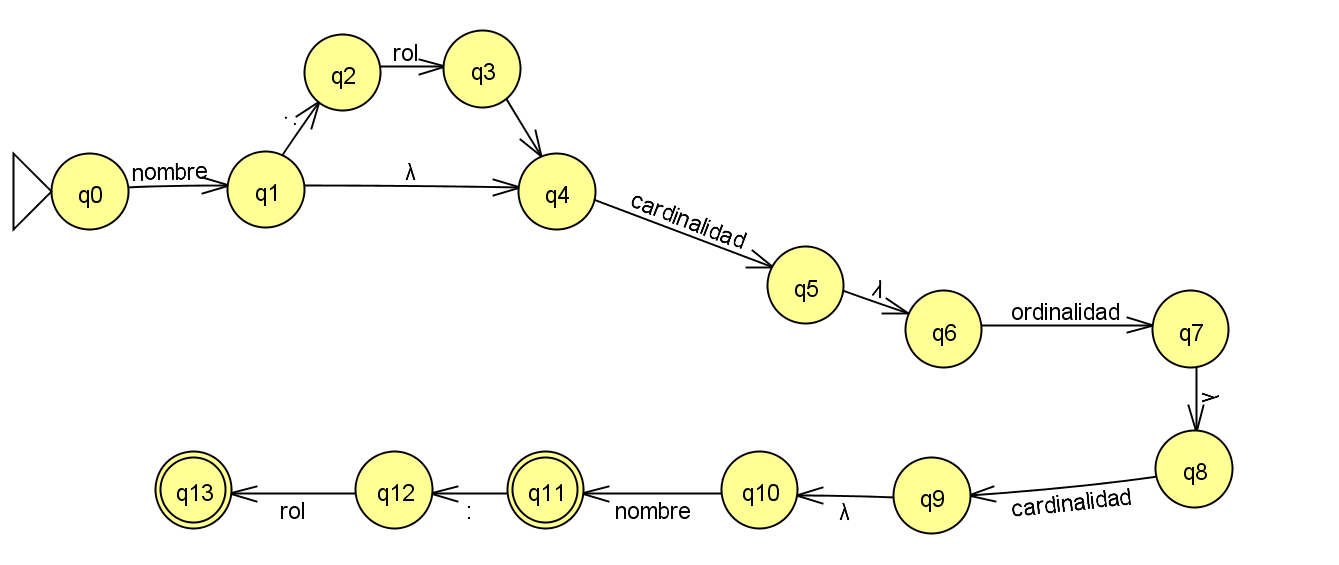
\includegraphics[width=.4\linewidth]{automatas_finitos/relacionDrt.png}
	\caption{Autómata finito - Relación}
	\label{fig:af_relacion}
\end{figure}

\subsection*{Definición \texttt{cardinalidad}}
\label{sub:cardinalidad}

Dentro de una relación la cardinalidad representa la cantidad con la que
participa la clase en esa asociación con otra clase, de esta manera se pueden
representar cuestiones como:

\begin{displayquote}
	\textit{(...) se pretende que el alumno pueda tener muchas materias (...)}
\end{displayquote}

Aquí es necesario relacionar dos entidades como ser las del \texttt{alumno} y
la de \texttt{materia} para poder representar lo que se solicita, la
cardinalidad en este caso es de \texttt{muchos a muchos}, por el hecho de que,
ademas de qe el alumno pueda tener muchas materias, a las materias pueden
concurrir muchos alumnos, es decir que la materia tambien puede tener asociada
muchos alumnos.

La notación BNF para una relación es la siguiente:

\begin{lstlisting}[caption={BNF - Cardinalidad para una Relación},basicstyle=\footnotesize\ttfamily]
	<cardinalidad> ::= "<digito|'*'> < " |'..' <digito|'*'>> "
\end{lstlisting}

\begin{figure}[H]
	\centering
	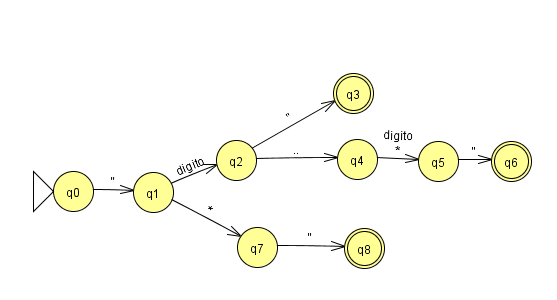
\includegraphics[width=.4\linewidth]{automatas_finitos/cardinalidadDrt.png}
	\caption{Autómata finito - Cardinalidad para una Relación}
	\label{fig:af_relacion_cardinalidad}
\end{figure}

\subsection*{Definicion \texttt{tipo-relacion}}
\label{sub:tiporelacion}

Este elemento, define como se relacionan las clases en una \texttt{relacion}
dada, por ejemplo, puede ser simplemente de \texttt{asociación} o se puede
tener una realcion de \texttt{herencia}.

Director maneja estas cuestiones con componentes que buscan el parecido a la
parte gráfica de los diagramas, por este motivo, estos tipos de relacion son
literales para cáda uno de los tipos que se necesite. A continuación se define
el BNF para el elemento en cuestión.

\begin{lstlisting}[caption={BNF - Tipos de Relación}, basicstyle=\footnotesize\ttfamily]
	<tipo-relacion> ::= <"<--"|"<|-"|"---"|"-|>"|"-->">
\end{lstlisting}

\begin{figure}[H]
	\centering
	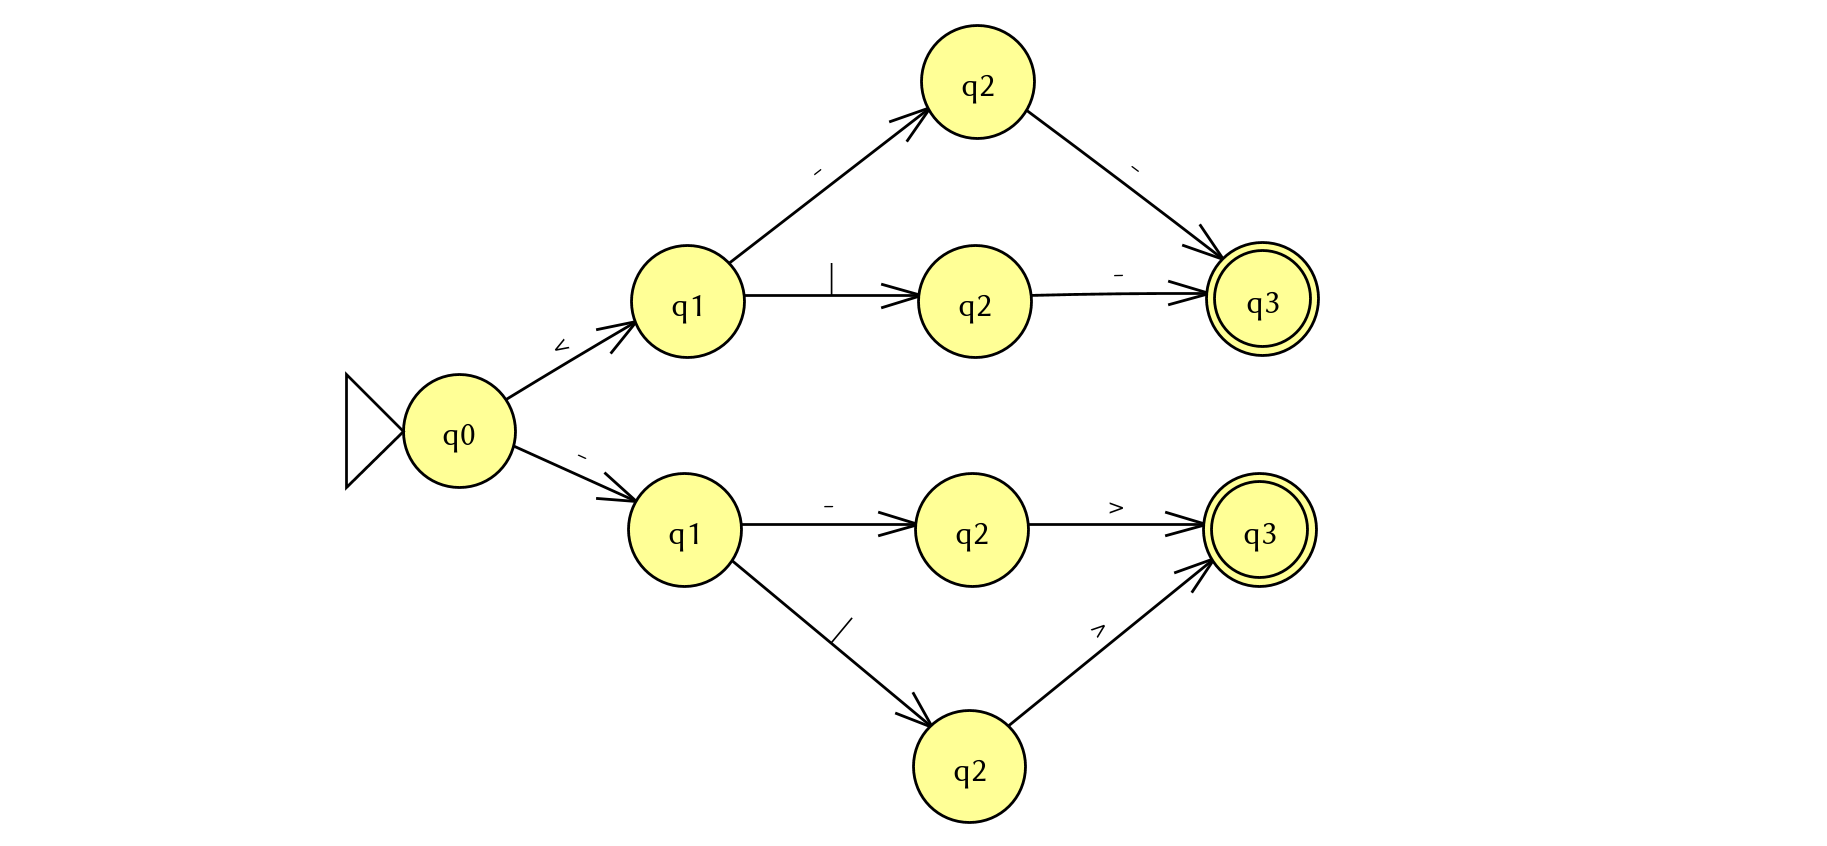
\includegraphics[width=.4\linewidth]{automatas_finitos/tipo-relacion.png}
	\caption{Autómata finito - Tipos de Relación}
	\label{fig:af_tipos_relaciones}
\end{figure}
